\documentclass{article}
\usepackage{styles/project_style} % Assuming you have this style file

\addbibresource{references/projects.bib} % Assuming bibliography file

% --- TITLE PAGE INFORMATION ---
\title{Introduction to the Forest Fire Model}

\begin{document}
\maketitle

\section{What is the Forest Fire Model?}

Picture a grid like a checkerboard, where each square (or ``cell'') can be empty, have a tree, or be on fire. The \textbf{Forest Fire Model (FFM)} is a computer simulation that acts like a game to show how fire spreads through a forest and how trees grow back over time. It’s a type of \textit{cellular automaton}, which is a fancy way of saying a model where simple rules for each square create complex patterns across the whole grid. Scientists use this model to study how small, local changes---like a single tree catching fire---can lead to big, system-wide effects, like massive wildfires.

The FFM was first developed by researchers like Bak, Chen, and Tang, and later improved by Drossel and Schwabl, to explore how simple rules can create complicated behaviors in nature. For example, it helps scientists understand how fires of different sizes happen or how dense a forest might become over time. The model mimics three key processes: fire spreading from tree to tree, new trees growing, and random events like lightning starting fires.

\begin{figure}[htbp]
  \centering
  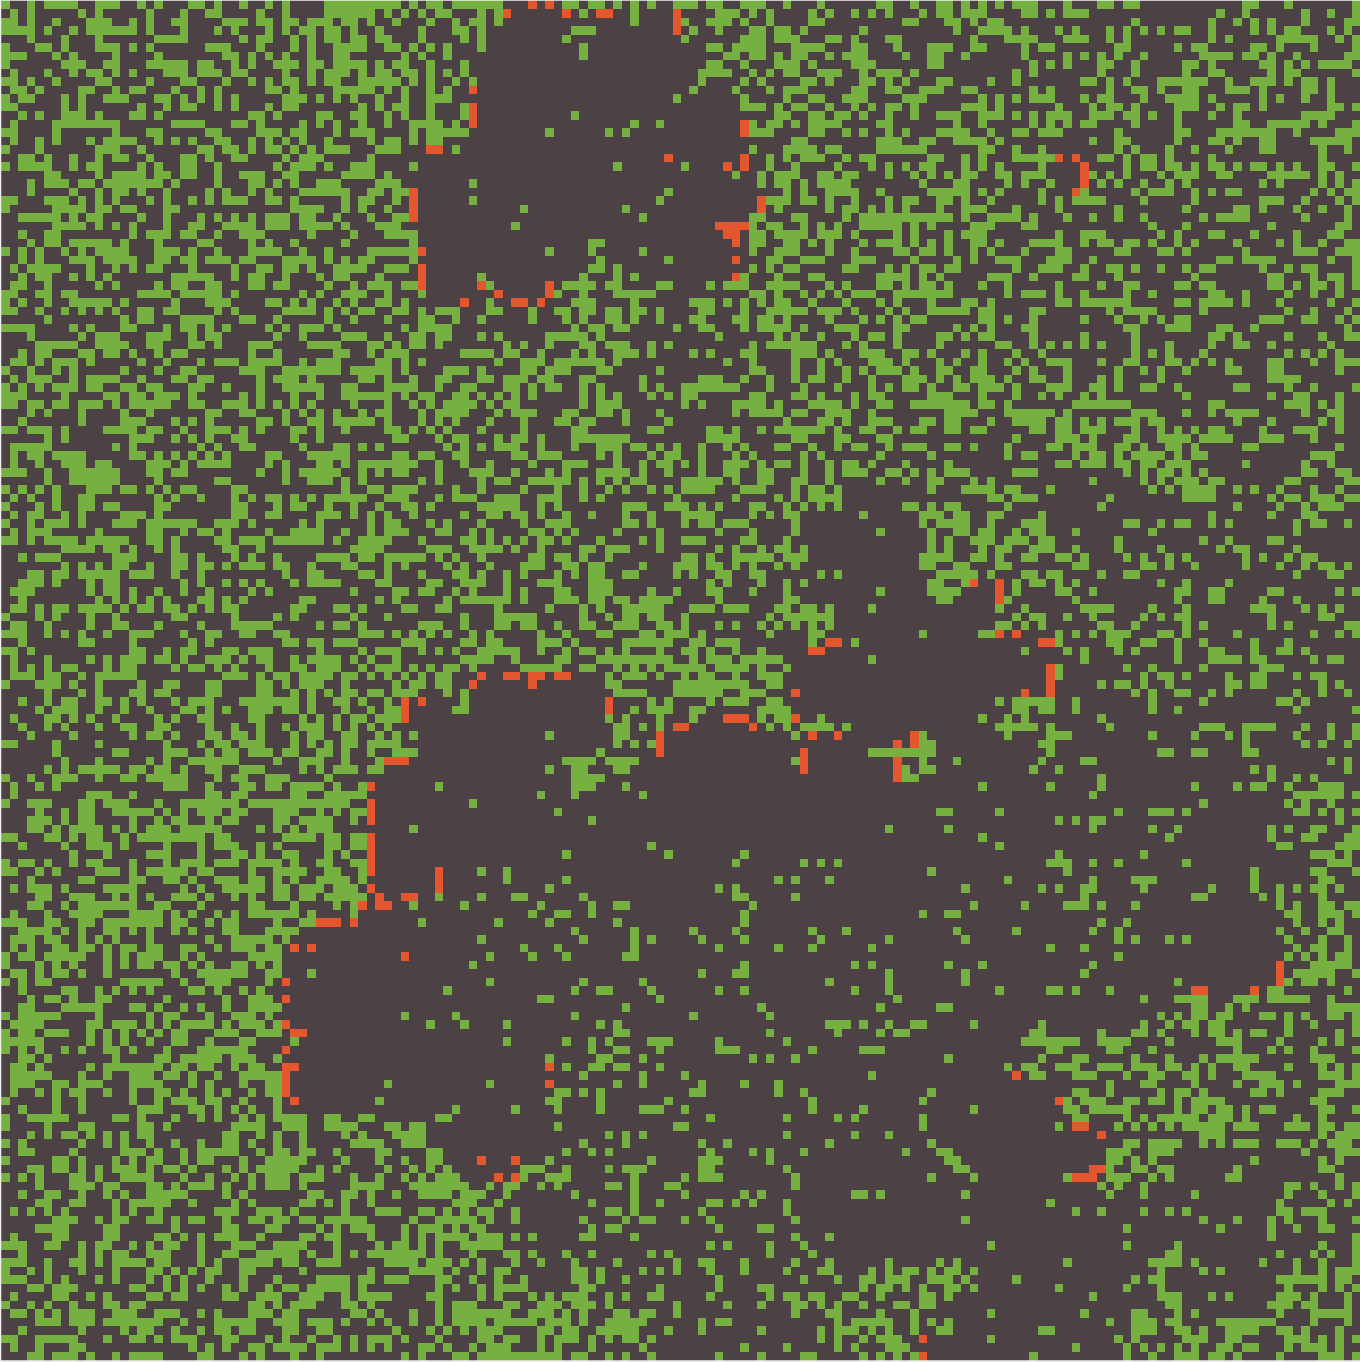
\includegraphics[width=0.4\textwidth]{projects/forest_fire/images/forest_fire.png}
  \caption{Illustration of the Forest Fire Model. Dark pixel represent ground, green pixel is vegetation and red pixel represent fire.}
  \label{fig:allee-effects}
\end{figure}


\subsection{Forest Fire Model vs. Wildfire Modeling}

The term ``Forest Fire Model'' can be confusing because it’s used in two different ways. In physics and math, the FFM refers to this simple, abstract grid-based model we’re talking about. It’s designed to study ideas, like how systems naturally organize themselves into a ``critical'' state where fires of all sizes can happen (a concept called \textbf{self-organized criticality}). But in real-world forestry and fire management, ``forest fire models'' or ``wildfire models'' (like FARSITE or BehavePlus) are much more detailed. These practical models include things like specific types of plants, hills and valleys, wind, humidity, and fire behavior to predict real wildfires accurately.

So, while the simple FFM is like a basic sketch to understand core ideas, real-world wildfire models are like detailed blueprints for actual forests. In the Capstone project, you should use basic Forest Fire Model as a starting point and add elements that lead to more physically realistic scenarions.

\subsection{How Does the FFM Work?}

Unlike some math models that use continuous equations (like those for population growth), the FFM works in a grid with discrete steps. Each square’s state---empty, tree, or fire---changes based on its own condition and what’s happening in the squares next to it. For example, a tree might catch fire if a neighboring square is burning, or an empty square might grow a new tree over time. These updates happen in time steps, like turns in a board game.

The FFM is a great way to explore how complex patterns, like unpredictable fire sizes, can come from simple rules. It’s especially useful for studying self-organized criticality, where a system naturally settles into a state where both small and huge events (like fires) can happen at any time.

\section{Key Components and Rules}

The model typically operates on a 2D lattice (grid). Each cell in the grid can exist in one of three states:
\begin{itemize}
    \item \textbf{Empty (or Ash):} Represents bare ground where a tree could potentially grow.
    \item \textbf{Tree (or Fuel):} Represents a living tree or flammable vegetation.
    \item \textbf{Burning:} Represents a tree that is currently on fire.
\end{itemize}

The system evolves in discrete time steps. During each step, the state of every cell is updated simultaneously (or sequentially in some implementations) based on the following rules (using the Drossel-Schwabl variant as a common example):

\begin{enumerate}
    \item \textbf{Burning Decay:} A cell that is currently \emph{Burning} becomes \emph{Empty} in the next time step (the fire consumes the fuel).
    \item \textbf{Fire Spread:} A \emph{Tree} cell becomes \emph{Burning} in the next time step if at least one of its immediate neighbors (e.g., the four von Neumann neighbors: North, South, East, West) is currently \emph{Burning}.
    \item \textbf{Lightning Strike (Spontaneous Ignition):} A \emph{Tree} cell that did not catch fire from a neighbor becomes \emph{Burning} with a small probability, $f$. This represents random ignition events like lightning.
    \item \textbf{Tree Growth:} An \emph{Empty} cell becomes a \emph{Tree} with a certain probability, $p$, in the next time step. This represents regrowth.
\end{enumerate}

The parameters $p$ (growth probability) and $f$ (lightning probability) control the overall dynamics of the system. Typically, $f$ is much smaller than $p$ ($f \ll p$).


\section{Why is the Forest Fire Model Important?}

Even though the Forest Fire Model (FFM) is simple, it creates fascinating and complex patterns, making it a powerful tool for understanding nature and science. Here’s why it matters:

\begin{itemize}
    \item \textbf{Showing Self-Organized Criticality (SOC):} The FFM is a classic example of a system that naturally settles into a ``critical'' state, where fires of all sizes can happen. Small fires are common, but huge, landscape-changing fires are possible too. This follows a pattern called a power-law, meaning the size of fires varies widely, all from simple rules without any outside tweaking.
    \item \textbf{Creating Complex Patterns:} The model shows how simple actions, like a fire spreading to a nearby tree, can lead to big, intricate results. For example, it can create jagged fire edges, changing forest densities, or patterns that look like they follow a mathematical recipe, even though they come from basic grid rules.
    \item \textbf{Understanding Ecosystems:} The FFM gives a simple way to think about real-world forests, like how fires shape landscapes, break up habitats, or help ecosystems change over time. It’s like a starting point for studying nature’s cycles.
    \item \textbf{Inspiring Real Wildfire Tools:} While the FFM is a basic sketch, its ideas---using a grid, tracking changes, and including random events like lightning---helped spark the creation of advanced wildfire models. These detailed tools predict real fires, assess risks, and guide forest management today.
    \item \textbf{Exploring Physics Ideas:} The model helps scientists study big concepts, like how systems shift from one state to another (think of a sparse forest with small fires versus a dense one with huge fires). It connects to ideas in physics about how things spread, like water soaking through a sponge.
    \item \textbf{Teaching Computer Simulations:} The FFM is a great example for learning how to build and study computer models. It’s like a fun, simple game that teaches students about cellular automata (grid-based simulations) and how to analyze complex systems.
\end{itemize}

By studying the FFM, we see how unpredictable events, like massive wildfires, might be a natural part of systems that are  on the edge of big changes. This idea is useful even when looking at more detailed wildfire models.

\section{Algorithmic Representation}

The simulation of the Forest Fire Model typically proceeds as follows:

\begin{enumerate}
    \item \textbf{Initialization:} Create a grid (e.g., an $L \times L$ matrix) and initialize the state of each cell, often starting with an empty grid or a random distribution of states.
    \item \textbf{Time Evolution Loop:} Repeat for a desired number of time steps:
        \begin{itemize}
            \item Create a new grid (e.g., `next\_grid`) of the same size to store the states for the next time step, typically initialized as a copy of the current grid or empty.
            \item \textbf{Iterate through each cell $(i, j)$ of the current grid:}
                \begin{itemize}
                    \item \textbf{Check Burning Cells:} If `current\_grid[i, j]` is \emph{Burning}, set `next\_grid[i, j]` to \emph{Empty}.
                    \item \textbf{Check Tree Cells:} If `current\_grid[i, j]` is \emph{Tree}:
                        \begin{itemize}
                            \item Check its neighbors in `current\_grid`. If any neighbor is \emph{Burning}, set `next\_grid[i, j]` to \emph{Burning}.
                            \item If no neighbor is burning, check for lightning: generate a random number $r \in [0, 1]$. If $r < f$, set `next\_grid[i, j]` to \emph{Burning}.
                            \item If no neighbor is burning and no lightning strike occurs, the cell remains a \emph{Tree} (i.e., `next\_grid[i, j]` stays \emph{Tree}).
                        \end{itemize}
                    \item \textbf{Check Empty Cells:} If `current\_grid[i, j]` is \emph{Empty}:
                        \begin{itemize}
                            \item Check for growth: generate a random number $r \in [0, 1]$. If $r < p$, set `next\_grid[i, j]` to \emph{Tree}.
                            \item Otherwise, it remains \emph{Empty} (`next\_grid[i, j]` stays \emph{Empty}).
                        \end{itemize}
                \end{itemize}
            \item \textbf{Update Grid:} Replace the `current\_grid` with the `next\_grid` for the next iteration.
            \item (Optional) Record data: Measure the size of active fires, density of trees, etc. Visualize the grid state.
        \end{itemize}
\end{enumerate}
*Note:* Careful implementation is needed regarding the order of updates, especially whether fire spread, lightning, and growth are evaluated based on the grid state at the beginning of the time step or potentially updated sequentially within the step. The simultaneous update described above (using a `next\_grid`) is common. Boundary conditions (e.g., periodic or fixed) also need to be defined.


\section{MATLAB Implementation Example}



\subsection{Model Parameters and Setup}
\begin{itemize}
    \item Grid States: $0$ = Empty, $1$ = Tree, $2$ = Burning
    \item $p$: Probability of tree growth (Empty $\to$ Tree)
    \item $f$: Probability of spontaneous ignition (Tree $\to$ Burning)
    \item `L`: Grid dimension ($L \times L$)
    \item `num\_steps`: Number of simulation steps
\end{itemize}

\subsection{MATLAB Code}
Matlab code for basic Forrest fire model.  Initiation sets parameters. 
\begin{lstlisting}[caption={Initial parameters}]
% --- Simulation Parameters ---
L = 160;             % Grid dimension
num_steps = 500;     % Number of simulation iterations
f = 0.00002;         % Probability of spontaneous ignition 
p = 0.004;           % Probability of tree growth 

% --- State Constants ---
EMPTY = 0;          
TREE = 1;           
BURNING = 2;        

% --- Initialization ---
grid = zeros(L, L);  % Initialize the grid as empty 

% --- Visualization Setup ---
figure(1);           % Create figure window
% Define colors for visualization
color_ground = [ 76  66  70] / 255; % Ground color
color_trees  = [118 176  65] / 255; % Tree color
color_fire   = [228  87  46] / 255; % Fire color
colormap([color_ground; color_trees; color_fire]); %

% Display initial grid and keep handle for updates
h_img = imagesc(grid); % Display initial grid and keep handle for updates
title(sprintf('Forest Fire Model - Step 0 / %d', num_steps));
axis equal off;      
clim([EMPTY BURNING]); 

\end{lstlisting}

The main loop Iterate through every cell in the current grid. It checks if any *neighbor* is burning (Moore neighborhood) and Calculate the next state based on rules and neighbor status using a helper function. It plots the result for each iteration.
\begin{lstlisting}[caption={Main code}]
for step = 1:num_steps
    % --- State Update ---
    next_grid = zeros(L, L); 
    for r = 1:L
        for c = 1:L 
            neighbor_is_burning = isNeighborBurning(r, c, grid, L, BURNING);
            current_state = grid(r, c);
            next_grid(r, c) = calculateNextState(current_state, neighbor_is_burning, p, f, EMPTY, TREE, BURNING);
        end
    end

    grid = next_grid; % Update the main grid with the calculated next states

    % --- Plotting ---
    set(h_img, 'CData', grid); % Update the displayed grid data
    title(sprintf('Forest Fire Model - Step %d / %d', step, num_steps));
    pause(0.05); 
end
\end{lstlisting}

There are two helper functions. First function  \texttt{isNeighborBurning} checks if the 8 Moore neighbors of the cell for fire. 

\begin{lstlisting}[caption={Helper functions}]
function is_burning = isNeighborBurning(r, c, grid, L, BURNING)
% neighbors).
    is_burning = false; % Assume no neighbor is burning initially
    % Iterate through the 3x3 neighborhood
    for dr = -1:1
        for dc = -1:1
            % Skip the center cell itself
            if dr == 0 && dc == 0
                continue;
            end
            % Calculate neighbor coordinates
            nr = r + dr;
            nc = c + dc;
            % Check if neighbor is within grid boundaries
            if nr >= 1 && nr <= L && nc >= 1 && nc <= L
                % If a neighbor is burning, set flag and exit loops
                if grid(nr, nc) == BURNING
                    is_burning = true;
                    return;
                end
            end
        end
    end
end

\end{lstlisting}

Function \texttt{calculateNextState} calculates the next state of a cell based on its current state, whether a neighbor is burning, and the growth/ignition probabilities. If cell is currently empty (ground) It becomes a tree with probability \texttt{p\_growth}.  If cell is currently a tree, it catches fire if a neighbor is burning OR it ignites spontaneously (lightning) with probability \texttt{f\_ignition}. If cell is currently burning It becomes empty in the next step (burns out).

\begin{lstlisting}[caption={Helper functions}]
function next_state = calculateNextState(current_state, neighbor_is_burning, p_growth, f_ignition, EMPTY, TREE, BURNING)
    switch current_state
        case EMPTY   % 
            if rand() < p_growth
                next_state = TREE;
            else
                next_state = EMPTY; % Stays empty otherwise
            end


        case TREE   
            random_ignition = rand() < f_ignition;
            if (neighbor_is_burning || random_ignition)
                next_state = BURNING; % Tree starts burning
            else
                next_state = TREE; % Stays a tree otherwise
            end
            
        case BURNING 
            next_state = EMPTY;
            
        otherwise 
            next_state = current_state; 
    end
end
\end{lstlisting}

\begin{itemize}
\item The code initializes a grid, usually predominantly trees.
\item It iterates through time steps, calculating the next state of each cell based on the rules and the current state of the grid and its neighbors.
\item Periodic boundary conditions ensure fire can wrap around the edges.
\item The imagesc function visualizes the grid state at each step, allowing observation of fire clusters spreading and dying out, and regrowth patterns.
\end{itemize}

\section{Example Scenario }

Running the simulation typically reveals characteristic dynamics:
\begin{itemize}
\item \textbf{Initial Transient:} If starting from a dense forest, large fires might initially sweep through until a balance is reached. If starting empty, the forest density gradually increases.
\item \textbf{Statistical Steady State:} After the transient phase, the system often reaches a fluctuating steady state. The overall density of trees fluctuates around an average value.
\item \textbf{Fire Dynamics:} Fires are constantly ignited by lightning. Most remain small and quickly burn out. Occasionally, a fire finds a large, connected cluster of trees and spreads significantly, sometimes clearing large areas of the grid.
\item \textbf{Self-Organized Criticality:} The key observation is that the distribution of the sizes of these fire clusters (e.g., measured by the number of cells burned in one event) often follows a \textbf{power law}, $P(s) \propto s^{-\tau}$, where $s$ is the size and $\tau$ is a characteristic exponent. This indicates scale-invariance: there's no typical fire size, and events of all magnitudes occur, driven purely by the internal dynamics. Large, "catastrophic" fires are rare but an intrinsic part of the system's behavior.
\item \textbf{Visual Patterns:} Observers can see fires propagating, often leaving behind complex, sometimes fractal-like boundaries between burnt and unburnt areas. Patches of regrowth appear in the empty areas.
\end{itemize}
This behavior contrasts with systems that might have a single characteristic scale or predictable, periodic behavior. The FFM shows how simple local rules generate complex, scale-free dynamics.

\section{Literature}
\subsection{General Introduction}
The Forest Fire Model is widely discussed in physics and complexity science literature. Online resources and textbooks on cellular automata or complex systems often cover it.
\begin{itemize}
% Replace these with actual keys from your projects.bib file
\item \href{https://en.wikipedia.org/wiki/Forest-fire_model}{Forest Fire Model (Wikipedia)}
\item \href{https://itp.uni-frankfurt.de/~gros/StudentProjects/Projects_2020/projekt_lars_dingeldein/}{A Cellular Automata Based Forest-Fire Model}
\end{itemize}

\subsection{Foundational Papers}
Seminal and related papers.
\begin{itemize}
    \item \textcite{ForestFire_Bak1990}
    \item \textcite{ForestFire_Chen1990}
    \item \textcite{ForestFire_Drossel1992}
\end{itemize}

\subsection{Journal Club Papers}
Suggested papers that for Journal Club presentation.
\begin{itemize}
    \item \textcite{ForestFire_Rui2017}
    \item \textcite{ForestFire_Zhou2025}
    \item \textcite{ForestFire_Zheng2017}
    \item \textcite{ForestFire_Mutthulakshmi2020}
    \item \textcite{ForestFire_Freire2019}
    \item \textcite{ForestFire_Alexandridis2008}
    \item \textcite{ForestFire_Mutthulakshmi2020}
    
\end{itemize}

\section{Conclusion}
The abstract Forest Fire Model, demonstrates  how a simple, local rules can generate complex, large-scale behavior characteristic of many natural systems. Its ability to exhibit self-organized criticality without fine-tuning parameters makes it a conceptual model for understanding phenomena ranging from literal wildfires to stock market crashes or disease epidemics. It demonstrates the importance of spatial structure, local interactions, and stochasticity in shaping system-level dynamics. While it is highly simplified compared to real ecosystems and current wildfire prediction tools, its core principles offer valuable insights into disturbance, resilience, and the emergence of complexity. 

\printbibliography % Command to print the bibliography defined in references/projects.bib

\end{document}